\subsubsection{bringit::server::usecase::GetListInfoUseCase}

\label{bringit::server::usecase::GetListInfoUseCase}
\begin{figure}[H]
	\centering
	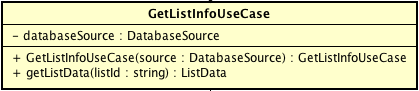
\includegraphics[scale=0.5]{Sezioni/SottosezioniST/img/app/GetListInfoUseCase.png}
	\caption{bringit::server::usecase::GetListInfoUseCase}
\end{figure}

\begin{itemize}
\item \textbf{Descrizione}: Classe di comunicazione con il database.
\item \textbf{Utilizzo}: La classe verrà utilizzata nel caso serva ricavare informazioni riguardanti una lista dal database.
\item \textbf{Attributi}: 
	\begin{itemize}
	\item \textit{private databaseSource:DatabaseSource}\\
	Il riferimento al database.
	\end{itemize}
\item \textbf{Metodi}:
	\begin{itemize}
	\item \textit{public GetListInfoUseCase():GetListInfoUseCase}\\
	Il costruttore della classe GetListInfoUseCase.
	\item \textit{public getListData(listId:Mongo.ObjectID):ListData}\\
	Questo metodo ritorna una la lista, recuperata dal database, corrispondente all'id passato come parametro.
				\\ \textbf{Parametri}: \begin{itemize}
			\item \textit{listId:Mongo.ObjectID}\\
			L'id della lista che si vuole recuperare dal database.
					\end{itemize} 
	\end{itemize}
\item \textbf{Eventi}:
\end{itemize}

\subsubsection{bringit::server::usecase::ManageListsUseCase}

\label{bringit::server::usecase::ManageListsUseCase}
\begin{figure}[H]
	\centering
	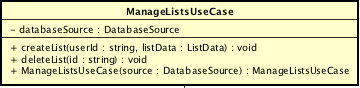
\includegraphics[scale=0.5]{Sezioni/SottosezioniST/img/app/ManageListsUseCase.png}
	\caption{bringit::server::usecase::ManageListsUseCase}
\end{figure}

\begin{itemize}
\item \textbf{Descrizione}: Classe di comunicazione con il database.
\item \textbf{Utilizzo}: La classe verrà utilizzata nel caso serva eliminare una lista dal database.
\item \textbf{Attributi}: 
	\begin{itemize}
	\item \textit{private databaseSource:DatabaseSource}\\
	Il riferimento al database.
	\end{itemize}
\item \textbf{Metodi}:
	\begin{itemize}
	\item \textit{public ManageListsUseCase():ManageListsUseCase}\\
	Il costruttore della classe ManageListsUseCase.
	\item \textit{public deleteList(listId:Mongo.ObjectID):void}\\
	Questo metodo rimuove la lista corrispondente all'id passato come parametro dal database.
				\\ \textbf{Parametri}: \begin{itemize}
			\item \textit{listId:Mongo.ObjectID}\\
			L'id della lista che si vuole rimuovere dal database.
					\end{itemize} 
	\end{itemize}
\item \textbf{Eventi}:
\end{itemize}
 
\subsubsection{bringit::server::usecase::ShareListUseCase}

\label{bringit::server::usecase::ShareListUseCase}
\begin{figure}[H]
	\centering
	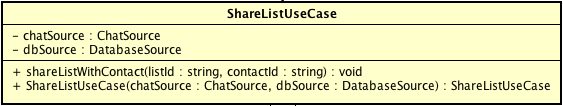
\includegraphics[scale=0.5]{Sezioni/SottosezioniST/img/app/ShareListUseCase.png}
	\caption{bringit::server::usecase::ShareListUseCase}
\end{figure}

\begin{itemize}
\item \textbf{Descrizione}: Classe di comunicazione con il database.
\item \textbf{Utilizzo}: La classe verrà utilizzata nel caso una lista venga condivisa con un'utente.
\item \textbf{Attributi}: 
	\begin{itemize}
	\item \textit{private databaseSource:DatabaseSource}\\
	Il riferimento al database.
	\end{itemize}
\item \textbf{Metodi}:
	\begin{itemize}
	\item \textit{public ShareListUseCase():ShareListUseCase}\\
	Il costruttore della classe ShareListUseCase.
	\item \textit{public shareListWithContact(listId:Mongo.ObjectID,contactId:string):void}\\
	Questo metodo salva la condivisione di una specifica lista con un utente.
				\\ \textbf{Parametri}: \begin{itemize}
			\item \textit{listId:Mongo.ObjectID}\\
			L'id della lista che si vuole condividere.
			\item \textit{contactId:string}\\
			L'id dell'utente al quale si vuole condividere la lista.
					\end{itemize} 
	\end{itemize}
\item \textbf{Eventi}:
\end{itemize}

\subsubsection{bringit::server::usecase::ModifyListUseCase}

\label{bringit::server::usecase::ModifyListUseCase}
\begin{figure}[H]
	\centering
	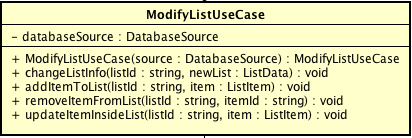
\includegraphics[scale=0.5]{Sezioni/SottosezioniST/img/app/ModifyListUseCase.png}
	\caption{bringit::server::usecase::ModifyListUseCase}
\end{figure}

\begin{itemize}
\item \textbf{Descrizione}: Classe di comunicazione con il database.
\item \textbf{Utilizzo}: La classe verrà utilizzata nel caso una lista venga modificata per salvare i cambiamenti di quest'ultima.
\item \textbf{Attributi}: 
	\begin{itemize}
	\item \textit{private databaseSource:DatabaseSource}\\
	Il riferimento al database.
	\end{itemize}
\item \textbf{Metodi}:
	\begin{itemize}
	\item \textit{public ModifyListUseCase():ModifyListUseCase}\\
	Il costruttore della classe ModifyListUseCase.
	\item \textit{public saveList(listId:Mongo.ObjectID):void}\\
	Questo metodo salva le modifiche a una lista se l'id passato come parametro è già presente nel database, altrimenti ne crea una nuova con id corrispondente.
				\\ \textbf{Parametri}: \begin{itemize}
			\item \textit{listId:Mongo.ObjectID}\\
			L'id della lista che si vuole modificare o creare.
					\end{itemize} 
	\item \textit{public addItem(listId:Mongo.ObjectID,item:ListItem):void}\\
	Questo metodo aggiunge un item a una lista nel database.
				\\ \textbf{Parametri}: \begin{itemize}
			\item \textit{listId:Mongo.ObjectID}\\
			L'id della lista alla quale si vuole aggiungere un prodotto.
			\item \textit{item:ListItem}\\
			Il prodotto che si vuole aggiungere.
					\end{itemize}
	\item \textit{public removeItem(listId:Mongo.ObjectID,item:ListItem):void}\\
	Questo metodo rimuove un item da una lista nel database.
				\\ \textbf{Parametri}: \begin{itemize}
			\item \textit{listId:Mongo.ObjectID}\\
			L'id della lista dalla quale si vuole rimuovere un prodotto.
			\item \textit{item:ListItem}\\
			Il prodotto che si vuole rimuovere.
					\end{itemize} 
	\item \textit{public updateItemInsideList(listId:Mongo.ObjectID,item:ListItem):void}\\
	Questo metodo aggiorna i dati di un item di una lista nel database.
				\\ \textbf{Parametri}: \begin{itemize}
			\item \textit{listId:Mongo.ObjectID}\\
			L'id della lista della quale si vuole aggiornare un prodotto.
			\item \textit{item:ListItem}\\
			Il prodotto che si vuole aggiornare.
					\end{itemize} 
	\end{itemize}
\item \textbf{Eventi}:
\end{itemize}